(Entnommen aus \glqq The Top 10 Algorithms in Data Mining\grqq~\cite{WuKumar2009}) \\[10pt]
Ein Datensatz besteht aus nur 4 Datenpunken:
$$
    \left\{
    \begin{array}{c}
        (x_1 =(0, +1), y_1=+1) \\
        (x_2 =(0, -1), y_2=+1) \\
        (x_3 =(+1, 0), y_3=-1) \\
        (x_4 =(-1, 0), y_4=-1)
    \end{array}
    \right\}
$$
\begin{figure*}
    \centering
    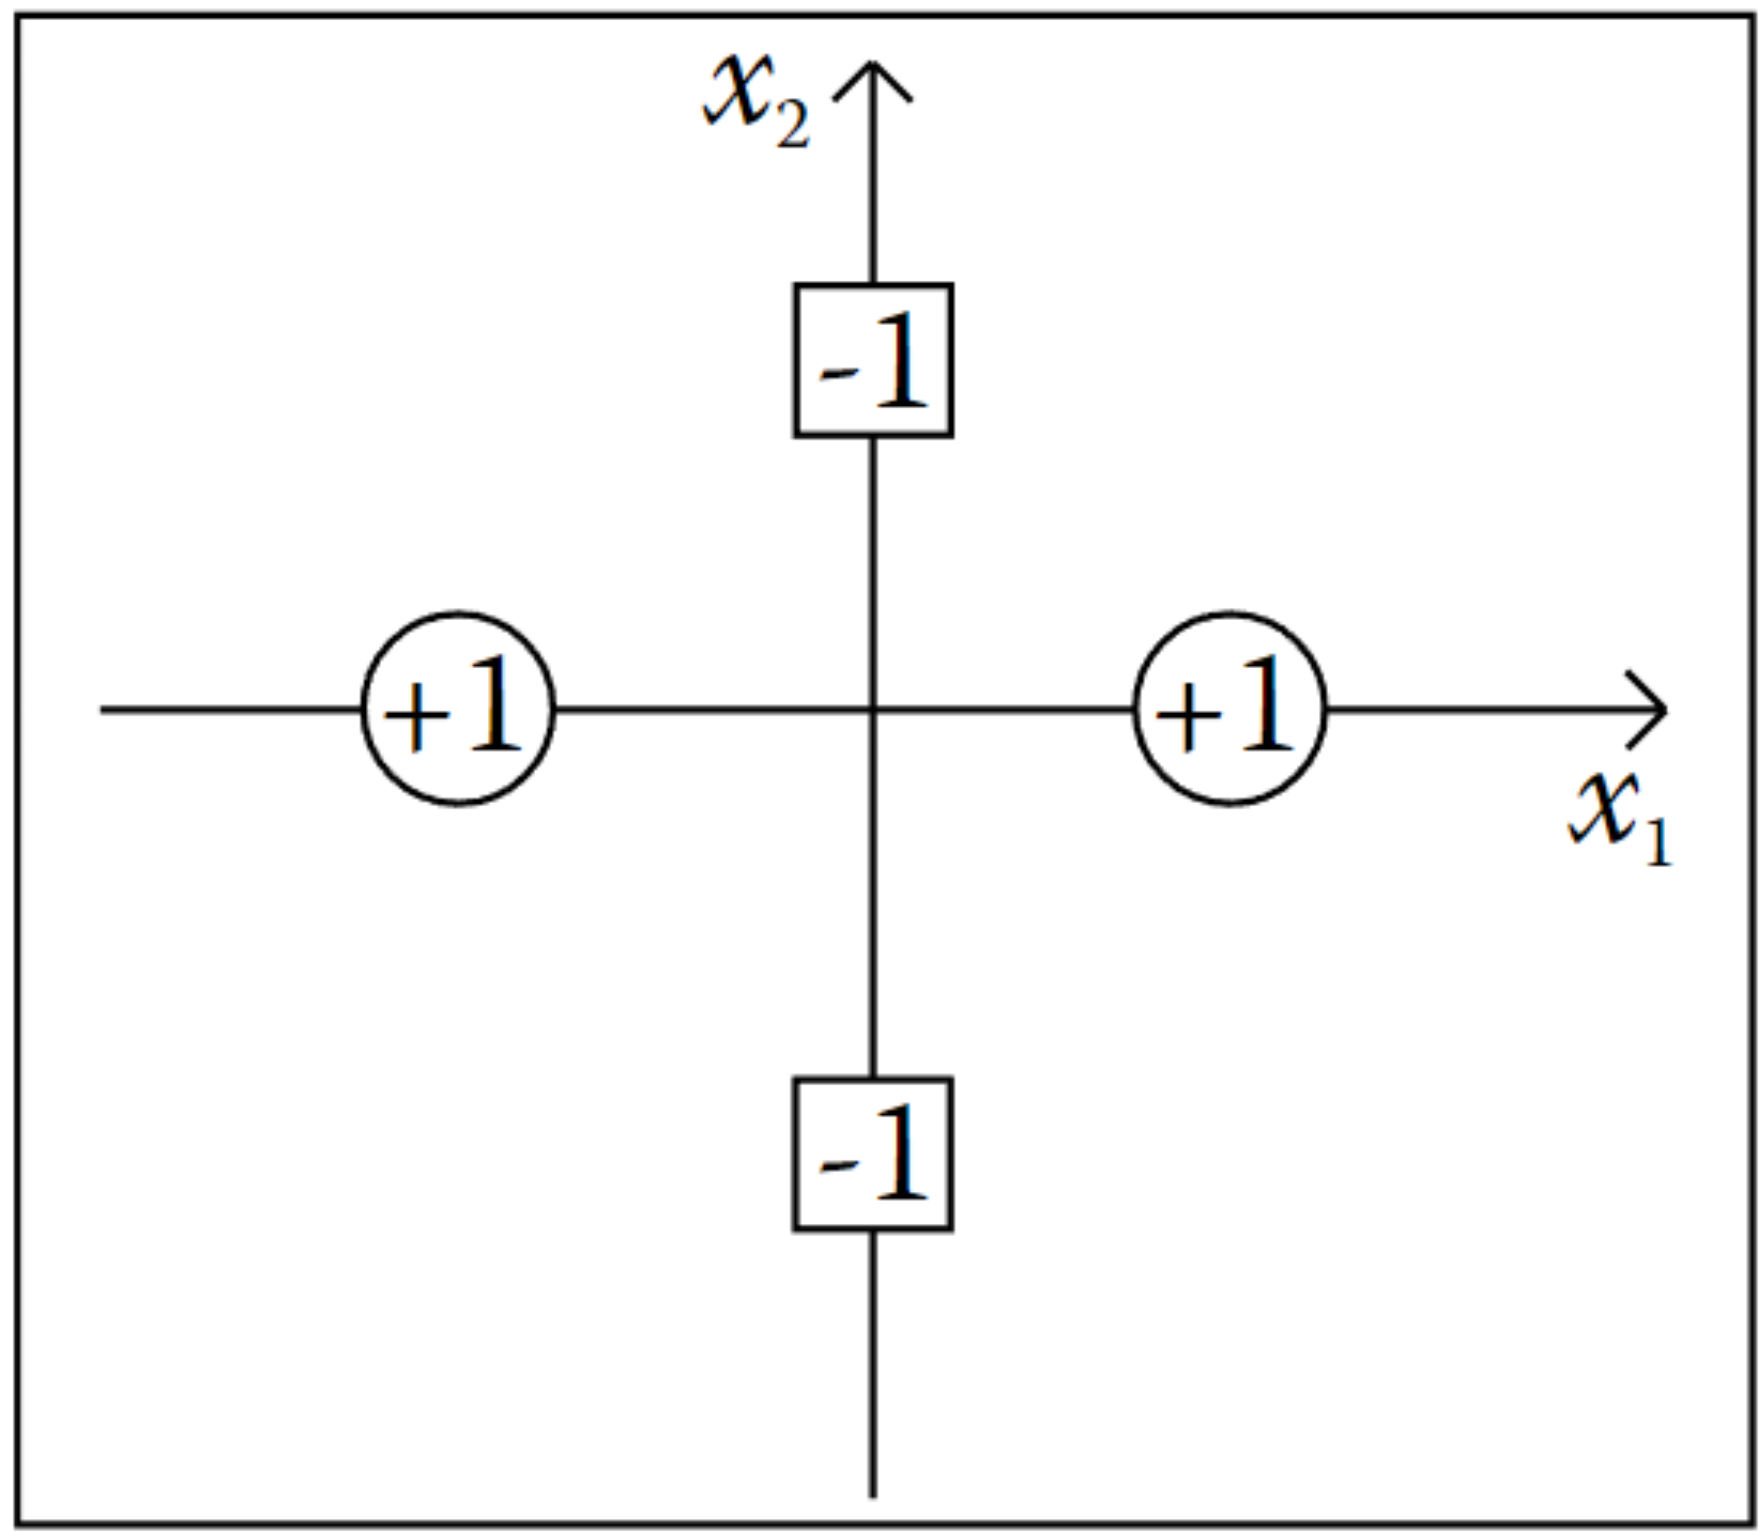
\includegraphics[width=0.5\textwidth]{figures/XOR-Problem.png}
    \caption[]{Visualisierung des XOR-Problems}
    \label{fig:XOR-Problem}
\end{figure*}
Wie aus Abbildung \ref*{fig:XOR-Problem} leicht zu erkennen ist, kann keine einfache Trennlinie gezogen werden, um
$+1$ und $-1$ voneinander zu trennen.\\
Nehmen wir nun an, dass durch den Lernalgorithmus nun acht Modelle als Funktionen vorliegen:
\begin{align*}
    h_1(x)=\left\{\begin{array}{r c}
                      +1, & \text{ wenn } (x_1 > -0.5) \\
                      -1, & \text{sonst}
                  \end{array}\right. &
    h_2(x)=\left\{\begin{array}{r c}
                      -1, & \text{ wenn } (x_1 > -0.5) \\
                      +1, & \text{sonst}
                  \end{array}\right. \\[10pt]
    h_3(x)=\left\{\begin{array}{r c}
                      +1, & \text{ wenn } (x_1 > +0.5) \\
                      -1, & \text{sonst}
                  \end{array}\right. &
    h_4(x)=\left\{\begin{array}{r c}
                      -1, & \text{ wenn } (x_1 > +0.5) \\
                      +1, & \text{sonst}
                  \end{array}\right. \\[10pt]
    h_5(x)=\left\{\begin{array}{r c}
                      +1, & \text{ wenn } (x_2 > -0.5) \\
                      -1, & \text{sonst}
                  \end{array}\right. &
    h_6(x)=\left\{\begin{array}{r c}
                      -1, & \text{ wenn } (x_2 > -0.5) \\
                      +1, & \text{sonst}
                  \end{array}\right. \\[10pt]
    h_7(x)=\left\{\begin{array}{r c}
                      +1, & \text{ wenn } (x_2 > +0.5) \\
                      -1, & \text{sonst}
                  \end{array}\right. &
    h_8(x)=\left\{\begin{array}{r c}
                      -1, & \text{ wenn } (x_2 > +0.5) \\
                      +1, & \text{sonst}
                  \end{array}\right. \\[10pt]
\end{align*}
\begin{enumerate}
    \item Der erste Schritt besteht darin, den Basis-Lernalgorithmus auf den ursprünglichen Daten aufzurufen.
          $h_2, h_3, h_5$ und $h_8$ haben alle eine Klassifikationsfehler von 0.25. Angenommen, $h_2$ wird als erster
          Basis-Lerner ausgewählt. Ein Datensatz $(x_1)$ wird falsch klassifiziert, daher beträgt der Fehler 0.25.
          Das Gewicht von $h_2$ beträgt ungefähr $\varepsilon_t\approx 0.55$. Abbildung \ref*{fig:XOR-Solution}(b) zeigt die Klassifikation und die Gewichtungen.
    \item Das Gewicht von $x_1$ wird erhöht und der Basis-Lernalgorithmus erneut aufgerufen. Diesmal haben $h_3, h_5$ und $h_8$
          gleiche Fehler. Angenommen, $h_3$ wird ausgewählt, dessen Gewicht 0.80 beträgt. Abbildung \ref*{fig:XOR-Solution}(c)
          zeigt die kombinierte Klassifikation von $h_2$ und $h_3$.
    \item Das Gewicht von $x_3$ wird erhöht. Diesmal haben nur $h_5$ und $h_8$ die niedrigsten Fehler. Angenommen, $h_5$ wird
          ausgewählt, dessen Gewicht 1.10 beträgt. Abbildung \ref*{fig:XOR-Solution}(d) zeigt die kombinierte Klassifikation
          von $h_2, h_3$ und $h_8$. Durch die Kombination der unvollkommenen linearen Klassifikatoren hat AdaBoost einen nichtlinearen Klassifikator mit
          null Fehler erzeugt.
\end{enumerate}
\begin{figure*}
    \centering
    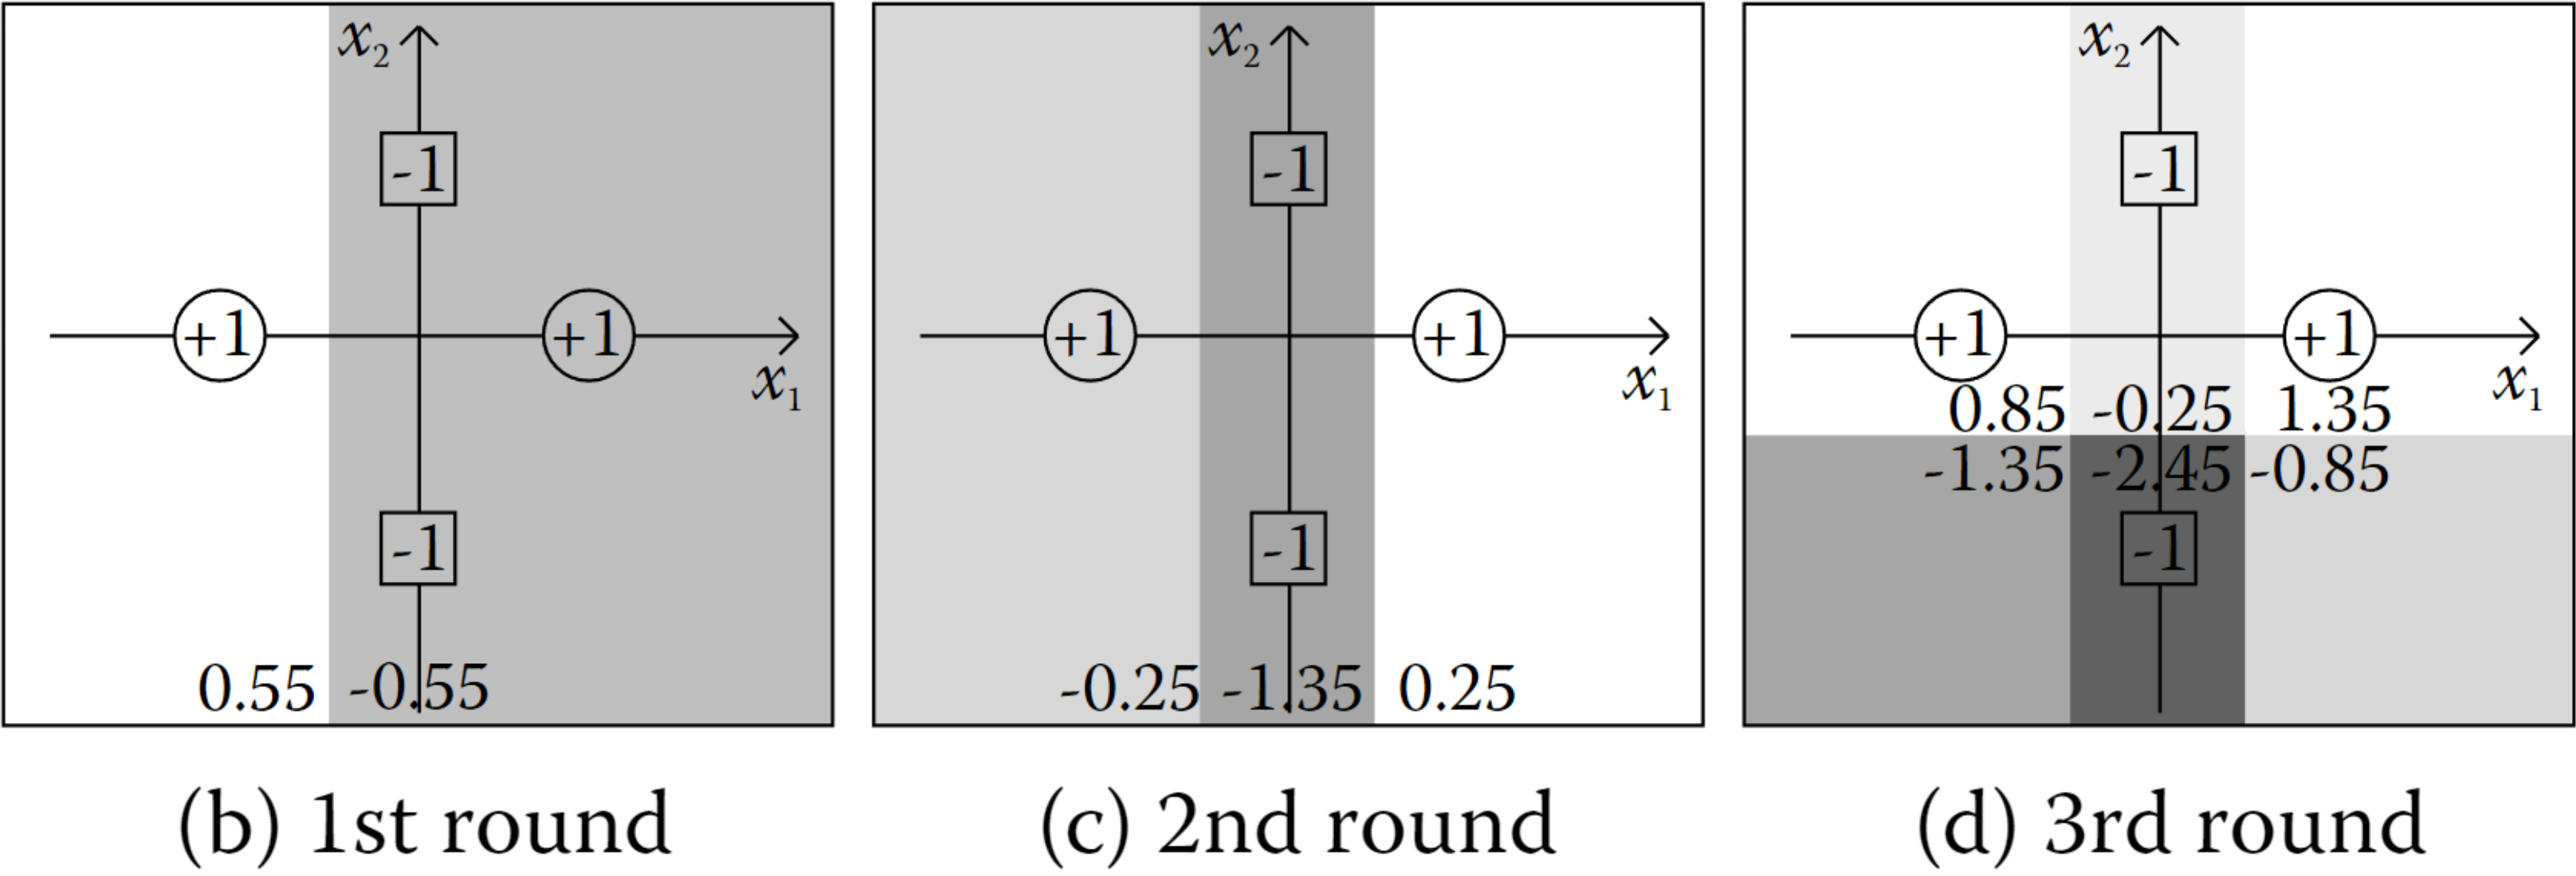
\includegraphics[width=0.7\textwidth]{figures/XOR_Solution.png}
    \caption[]{Visualisierung von AdaBoost auf dem XOR-Problem}
    \label{fig:XOR-Solution}
\end{figure*}